\section{Generative Modeling 3}
\subsection{Generative Adversarial Networks}
\begin{figure}[!h]
    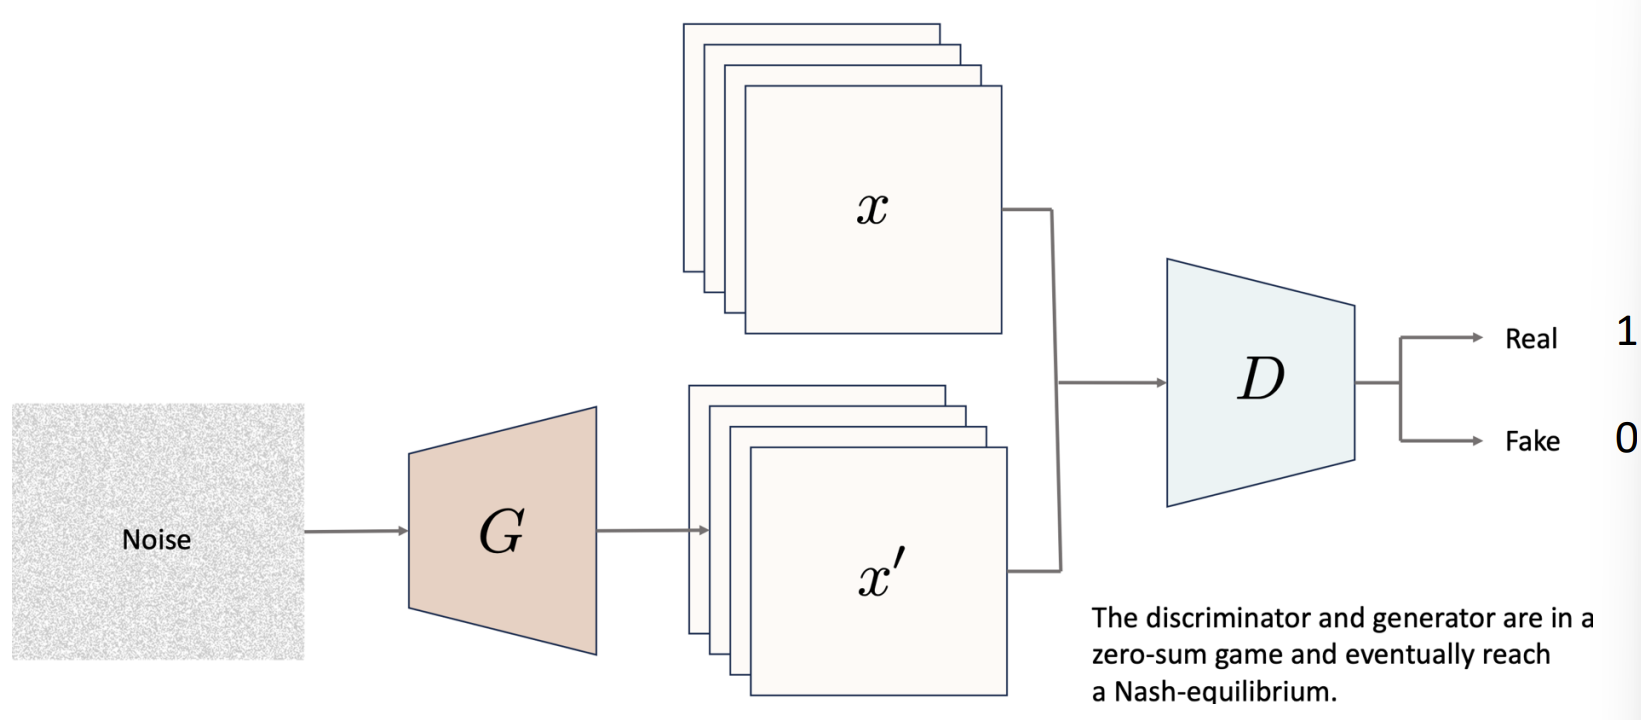
\includegraphics[width = \columnwidth]{figures/GenAI3/GAN.png}
\end{figure}
Definition: GANs are a framework where two networks compete: a generator G and a discriminator D 

GANs make no attempt to calculate or approximate the likelihood function!

G learns to generate images from latent space.

D learns to distinguish between real and fake.

Models compete and improve one another.

\begin{enumerate}
    \item Sample a latent noise vector
    \item Generate an image from the noise
    \item Sample real data
    \item Try too correctly guess real and fake data
\end{enumerate}
\[
\min_G \max_D \mathbb{E}_{x\sim p_{data}}\left[\text{log}D(x)\right] + \mathbb{E}_{z\sim p_{z}}\left[\text{log}(1-D(G(z)))\right]
\]

\subsubsection*{Generator's objectiv}
Minimize the above exression.
This means fooling the Discriminator network by making realistic images.

This is accomplished if D(G(z)) = 1, i.e., we fool \(D\) always predict our fake images as real.

Makes sense because if \(D(G(z)) = 1\), then the second expression is smallest if the log argument = 0.

\subsection*{Discriminator's objectiv}
Maximize the aboce expression.
This means correctly labelling images as real or fake.

This is accomplished if \(\text{log}D(x) = 1\) and \(D(G(z)) = 0\).
Makes sense because if \(\text{log}D(x) = 1\) is the largest value for given range \(\left[ 0,1\right]\) and the second term is largest for log\((1)\),i.e.,\(D(G(z)) = 0\).

\subsubsection{Training}
\begin{figure}[!h]
    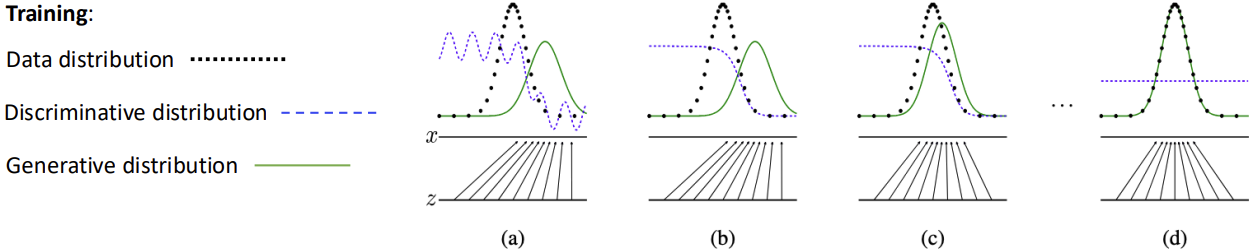
\includegraphics[width = \columnwidth]{figures/GenAI3/TrainingGAN.png}
\end{figure}

\begin{enumerate}[label = (\alph*)]
    \item Partly converged adversarial pair. D better than guess.
    \item D is updated during inner loop \(D^*(x) = p_{data} /(p_{data}(x)+p_g(x))\) and converges, resulting in a better classification.
    \item The gradient from D the guid \(G(z)\) to flow to regions more likely to be classified as real data (at optimality tries to minimize the JS Divergence)
    \item After several iterations discriminator cannot distinguish between distributions in \(D(x) = \frac{1}{2}\).
\end{enumerate}

Why does \(p_g \rightarrow p_{data}\):
\begin{enumerate}
    \item When solving for optimal \(D\) we can take the derivative of 
    \[
    \mathcal{L}_D = \int p_{data}(x) \text{log}D(x)dx + \int p_g(x)\text{log}(1-D(x))dx.
    \]
    Set the expression = 0 and solve for \(D\).
    \item This gives the optimal behaviour of \(D\) for a fixed generator as \(D^*(x) = \frac{p_{data}(x)}{p_{data}(x) + p_g(x)}\)
    \subitem When \(p_{data}(x) >> p_g(x) : D^*(x) \approx 1\), x is classified as real
    \subitem When \(p_{g}(x) >> p_{data}(x) : D^*(x) \approx 0\), x is classified as fake
    \subitem When \(p_{data}(x) = p_g(x) : D^*(x) = 0.5\), the discriminator becomes uncertain because \(D\) is producing realistic images
    \item If we substitute \(D^*(x)\) into the GAN objective, we see that GAN indirectly minimizes \(JS(P||Q) = \frac{1}{2}\text{KL}(P||M) +\frac{1}{2}\text{KL}(Q||M) \)
\end{enumerate}

\textbf{Equilibrium}: GANs in theory should reach an equilibrium called a Nash equilibrium (a situation where no player could gain by changing their own strategy).
This means indirectly minimizing the Jenson-Shanon(JS) divergence.
This is a smoothed symmetric version of the KL-divergence.
\[
JS(P||Q) = \frac{1}{2}\text{KL}(P||M) +\frac{1}{2}\text{KL}(Q||M)
\]
Where \(P\) and \(Q\) are the real and generated distributions and \(M\) is the midpoint or mixture distribution\((P+Q)/2\).

At equilibrium, the \(p_{data} = p_g\) and the discriminator
\[
D(X) = \frac{p_{data}(x)}{p_{data}(x) + p_g(x)}
\]
should output a \(0.5\).

\subsubsection{Problems with GANs}
\begin{enumerate}
    \item Zero Gradient information if \(D\) is too powerful (common at start).
    \item Mode collapse: When \(G\) finds a solution by generating the same image, this induces and undesirable quality of a non bijective map.
\end{enumerate}
\subsection{DCGANs}
\begin{enumerate}
    \item Combine CNN with GAN, both in the \(D\) and \(G\) networks
    \item Upscale using transpose Convs 
    \item Batch Normalization, Leaky ReLU in \(D\)m ReLU in \(G\)
\end{enumerate}
Much better generative results, still far from perfect.

\subsection{Conditional GANs(cGAN)}